\chapter{Introduction}
\label{chap:Introduction}
This chapter introduces IT minds, which the project is made in collaboration
with. It also explains why the project is made, and defines the problem
definition. Lastly it explains the structure of the report. 

\section{IT minds}
\label{sec:IT minds}
IT minds is a Danish software consultant company\cite{IT-minds}, who primarily
employ students to solve the consultant tasks they get. The idea is that
students of a software oriented study is capable of making software for
companies, but may lack the experience to get hired after the education is done.
On top of that since the developers are under education the customers don't have
to pay as much as for someone who is done with their study, and therefore some
money can be saved. 

It started in Århus, and later an office was opened in Copenhagen, this means
that systems used internally cannot be based on a local network without a setup
like a VPN, and as the company does not host anything themselves there are no
servers to host a system with a VPN. This means that most systems are based on
internet solutions, with separate user login. 

Many of the customers of IT minds wants things made in C\# as that allows then
to take over the code afterwards, and it means that they can use their existing
echo systems. This results in a lot of the developers in IT minds knowing C\#,
or quickly pick it op. For this reason I have chosen to develop in the same
language, allowing other developers to take over and maintain it later. 

\section{Motivation}
\label{sec:Motivation}
Companies that rely on selling to other companies generally need a way to keep
track of what customers they have, and which customers they can potentially have
in the future. IT minds is an example of such a company. They do have a system
that keeps track of customer relations already, but it does not support all the
use cases that they want, and cannot give the information they are interested
in. Because of this they have asked me to make a new system to handle these
cases, since they do know that the time available is limited, the system will
not be a fully fetched one, but focus on the irritations they have with the
current systems, as well as the basic requirements for the system to work. 

A CRM\footnote{Customer Relation Management} system aims to allow a user to keep
track of what business agreements are currently active, as well as what could in
future be if all goes as planned. It can also allow the user to keep track of
who to contact under a customer, in case the customer is a company, or an
organization. 

Such a system could be run locally, but that reduces its usability, in that it
will be only a single person in the company, or a single machine that will be
able to keep track of the given information. Because of this a CRM is often run
as a web server, either on the local network of the company, or on the internet
so that it can be accessed from anywhere, which can be useful if the company has
multiple departments, or if the user wants to access it from a phone, or some
other device that may not be connected directly to the network the CRM is hosted
on, or have access to a VPN. 

It is not uncommon for a sales department to want to look up the contact
information of a client when they are not in the office, and for a company such
as IT minds with more than one department the need for a distributed system is
needed, this would generally be on a web server accessed via the internet. 

Even after we have figured out that we want the system to be run on a web server
we still have different ways to go, each with their own advantages and
disadvantages. Some of them could be writing a static website that is closely
connected to the server, so the server generates the appropriate HTML allowing
for communication with the database, via technologies such as php, JSP, or ASP.
Another way could be to write a web-api, serving the information only in raw
format on designated paths. A third option could be to make a
SOAP\footnote{Simple Object Access Protocol} web service, and access the
information via that. All this topic is discussed in further detail in
chapter~\ref{chap:Technology}. 

In figure~\ref{fig:sys_example} an example of how a system capable of showing
graphs could look. This is a screenshot taken at the end of the development
process, of the count of activities in a certain category, within a certain time interval.

\begin{figure}[h]
\centering
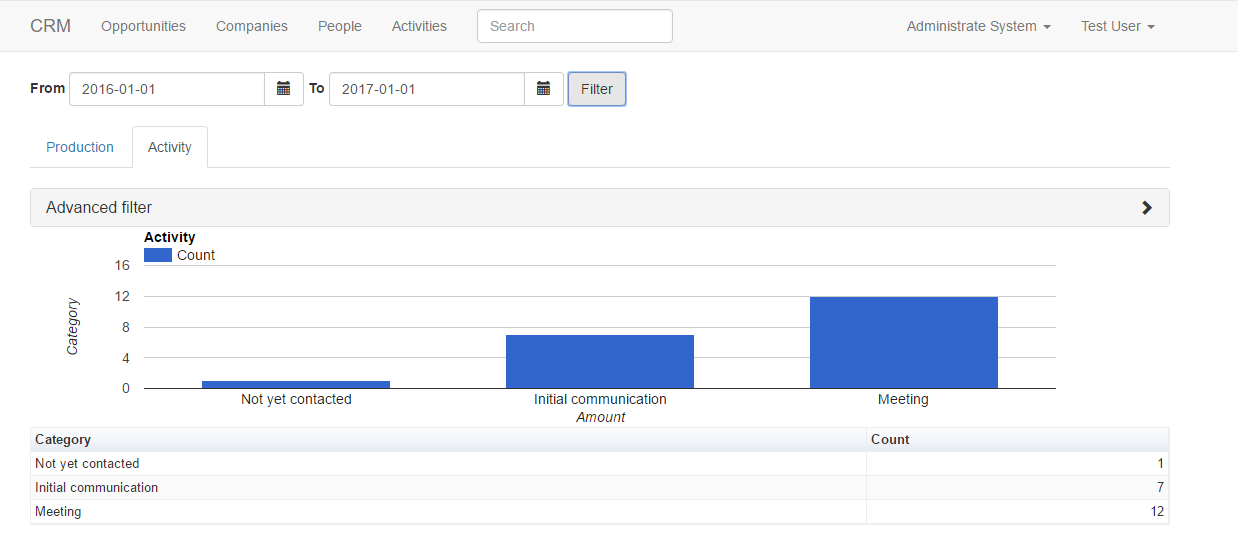
\includegraphics[width=\textwidth]{Mockups/screen_shots/activity_graph}
\caption{Example of how the system could look}
\label{fig:sys_example}
\end{figure}

\section{Vision}
\label{sec:Vision}
The vision of this project is to develop an alternate CRM for companies to use
that will focus on some of the missing features of other CRMs in regards to data
extraction. By making it a web service the accessibility will be improved, and
usage may be increased. The system will consist of only a subset of the full
feature set of other CRMs in addition to the other focuses. 

\section{Problem definition}
\label{sec:Problem definition}
A CRMs purpose is to allow the user to keep track of companies and people, and
who users on the CRM interact with the companies and people. This means that
there is a lot of room for specialization. The problem with this specialization
is that not any of the existing CRMs, at least that IT minds have tried cover
all the features they need. 

What is needed is the basic CRM features, and on top of that the ability to set
a production goal for each user of the CRM, giving a more clear incentive for
the user to do better, and promoting competition among the users. 

In some systems, eg. PipelineDeals\cite{pipelinedeals:features} this feature is
supported to some extend, but not in a way that makes sense for a company like
IT minds. What they really want, is to be able to make a per month goal, and
then have the ability to change that goal in the future. This goal feature
should be a per user thing, but one thing that is more important for the people
who manages the system than an individual user overview is a department, or
company overview, allowing them to see that the company is eg. 200.000 kr. away
from their goal next month, which if that trend keeps up may warrant a
reevaluation of methods. 

First I will do an analysis of the project, making the idea of the system
concrete, I will also in this phase determine the technologies that will be used
to build the system. These choices will be made based on communication with IT
minds as to make sure the system that is produces lives up to their
expectations, as well as allowing the common developer in IT minds to extend the
feature set, and maintain the system in the future if needed. This means the
language the system will be written is is going to be C\#, as most of the
software IT minds makes is written in C\#, an therefore most will be familiar
with it. 

In the design phase the design of the database, and the system will be made, so
that it is ready for the next phase, which is the implementation. It is in the
implementation phase the system will be implemented, and tested. In the end the
final testing phase will be entered, and the system will be tested more
thoroughly than it was in the development phase, to hopefully catch any bugs
there may be left. 

\subsection{Delimitation's}
\label{sub:Delimitations}
Because of the time available for the development of the project, and the size
of a full CRM I am forced to implement only a subset of all the features a
production ready CRM would consist of. As the primary focus of this project is
to create the backing structure for a CRM that supports the requested features,
the focus on a front-end, and the user experience will be lower. Some
implementation of visualization will be made as it is what the system is meant
to serve, but the primary focus will be on the collection, and manipulation of
the data as well as the ability to get it out again in a useful way. 

The primary product of the project will be a system that has the most essential
features of a CRM, but it will still be missing a lot of the features that makes
a full product convenient to use. This is because of the limitation in hours
that can be put into creating the system, which can be seen in that there are
companies who's primary product is a CRM, such as PipelineDeals. 

This also means that one of the aims of the project is to make sure that the
structure supports the addition of new features for further development, as that
will be needed in case it is going to be used actively. 

The report will not focus on the reasons of a lot of the data that the system
will be able to give the user, as that falls under different focus points than
software design, and implementation. It will not consider any legal issues in
regards to storing of personal data, or any issues regarding the possibility of
earning money off of it, since these are not of technical importance. 

\section{Development methods}
\label{sec:Development methods}
The development of this project will follow the method Kanban. The idea of this
method is to deal with the fact that customers change their minds during
development, and the development of the software therefore needs to follow a
more agile process in order to adjust to the changing requirements throughout
the process. 

The focus of Kanban is to make deliveries in a just-in-time fashion, where the
developers take the tasks from a queue of defined tasks. The tasks are usually
set up on a Kanban board, with has three primary columns, one for each state a
task can be in: 

\begin{center}
  $TODO \rightarrow Doing \rightarrow Done$
\end{center}

This is however only a sub board in a bigger environment, where we also could
have an analysis part and a test part. Which would allow for isolation of
bottlenecks\cite{kanban}. 

To keep track of this board I will be using the web application
PivotalTracker\footnote{Read more about PivotalTracker at:
  https://www.pivotaltracker.com}, which allows me to write user stories that
will describe what a user should be able to do, and by that describes the
functionality of the program, when I start work on a stories I will then move
the state as to indicate what I am working on. This state change represents the
moving from todo to doing, and finally to done. The values used in
PivotalTracker are: 

\begin{center}
  $Unstarted \rightarrow Started \rightarrow Finished$
\end{center}

There are a few other states PivotalTracker supports, but I will not be using
those. 

I will try to keep the development in iterations of two week intervals, which
means that every other week I will look at what I have done the past weeks, and define
what should be done the coming week. This process will involve Kristian Larsen
who is the Product owner in this context, representing IT minds and their
interests. The reason for the iterations is to keep the agile workflow, allowing
for changes put forth by Kristian when he sees the different stages of the
product. 

For the development of the features them selves, I will be following a
test-driven development procedure, meaning I will start by creating unit tests
for the feature I am to implement, which will fail until I the feature is done,
and supports the requirements. This will ensure quality code, as well as make
sure that the requirements are met throughout the product. 

\section{Goals}
\label{sec:Goals}
Based on the problem definition in section~\ref{sec:Problem definition} I will
now list the goals that will be carried out throughout the project, both in
regards to the report and the implementation of the product. 

\begin{enumerate}
  \item Introduce the problem
  \item Define the project, and decide what should be in the first delivery
  \item Decide what features must be supported for the CRM to be usable
  \item Define use cases the system should support
  \item Make a domain model describing the domain of the system
  \item Decide on a fitting database technology to store the data
  \item Decide on a fitting set of technologies to serve the data
  \item Describe what architecture the system is going to follow
  \item Design the database structure
  \item Decide on what design patterns to use for the project
  \item Implement the database from the designed structure
  \item Implement the application with the decided upon technologies
  \item Make a front-end implementation to communicate with the server
  \item Test the system using unit tests and integration tests
  \item Discuss the advantages and disadvantages of the testing
  \item Reflect on the resulting product, and what is missing compared to a full CRM
  \item Figure out future work for the product
\end{enumerate}

\section{Thesis structure}
\label{sec:Thesis structure}
Here I will go over the general structure of the report, and what each of the
chapters will focus on, as well as what goal they will complete.\\ 

\textbf{Chapter~\ref{chap:Domain analasys} - \nameref{chap:Domain analysis}}
will describe the domain the solution is under, including requirements from IT
minds to the solution, and a prioritized order of features that may be
implemented into the system. The chapter will also set up some use cases that
describe what a user might do in the system, and what should be supported by the
final product. 

\textbf{Covers goals: 2-5}\\

\textbf{Chapter~\ref{chap:Technology} - \nameref{chap:Technology}} will look at
some of the technologies that are available for developing the system, and make
a decision from the findings of this on what technologies will be used to
implement the system it self. 

\textbf{Covers goals: 6-7}\\

\textbf{Chapter~\ref{chap:Design} - \nameref{chap:Design}} will focus on the
design of the system itself, including the database design, and the architecture
of the system. It will also decide what design patterns will be used under the
development. 

\textbf{Covers goals: 8-10}\\

\textbf{Chapter~\ref{chap:Implementation} - \nameref{chap:Implementation}} will
discuss the implementation itself, including some of the design decisions made
while developing and the technologies that was chosen based on the previous
chapter. 

It will also go over how testing of the system has been done, including unit
tests, and integration tests. 

\textbf{Covers goals: 11-15}\\


\textbf{Chapter~\ref{chap:Conclusion} - \nameref{chap:Conclusion}} will hold the
final product up against the requirements, and a conclusion will be drawn from
the project. Future development of the product will also be discussed in this
chapter. It will end with a statement from IT minds.

\textbf{Covers goal: 16-17}
